%!TEX TS-program = xelatex
%!TEX root = ../../maxwell2018thesis.tex

\chapter[Result Diversification and Stopping Behaviour]{Result Diversification and\\Stopping Behaviour}\label{chap:diversity}
A searcher, when developing an information need, will often possess an incomplete mental model of the topic. As such, they may arrive at a retrieval system with an \emph{Anomalous State of Knowledge (ASK)}~\citep{belkin1980ask}. To address this deficiency in their mental model, a searcher will often issue a variety of different queries to explore the topic space~\citep{kelly2015search_tasks}. Often, such topics are \emph{aspectual} in nature, where an underlying goal is to find out about the different facets, dimensions of aspects of the topic. An example of aspects within a topic is illustrated below, taken from TREC Robust Track~\citep{voorhees2006trec_robust} topic 347.

\begin{figure}[h]
    \centering
    \vspace{4mm}
    \resizebox{1\hsize}{!}{
    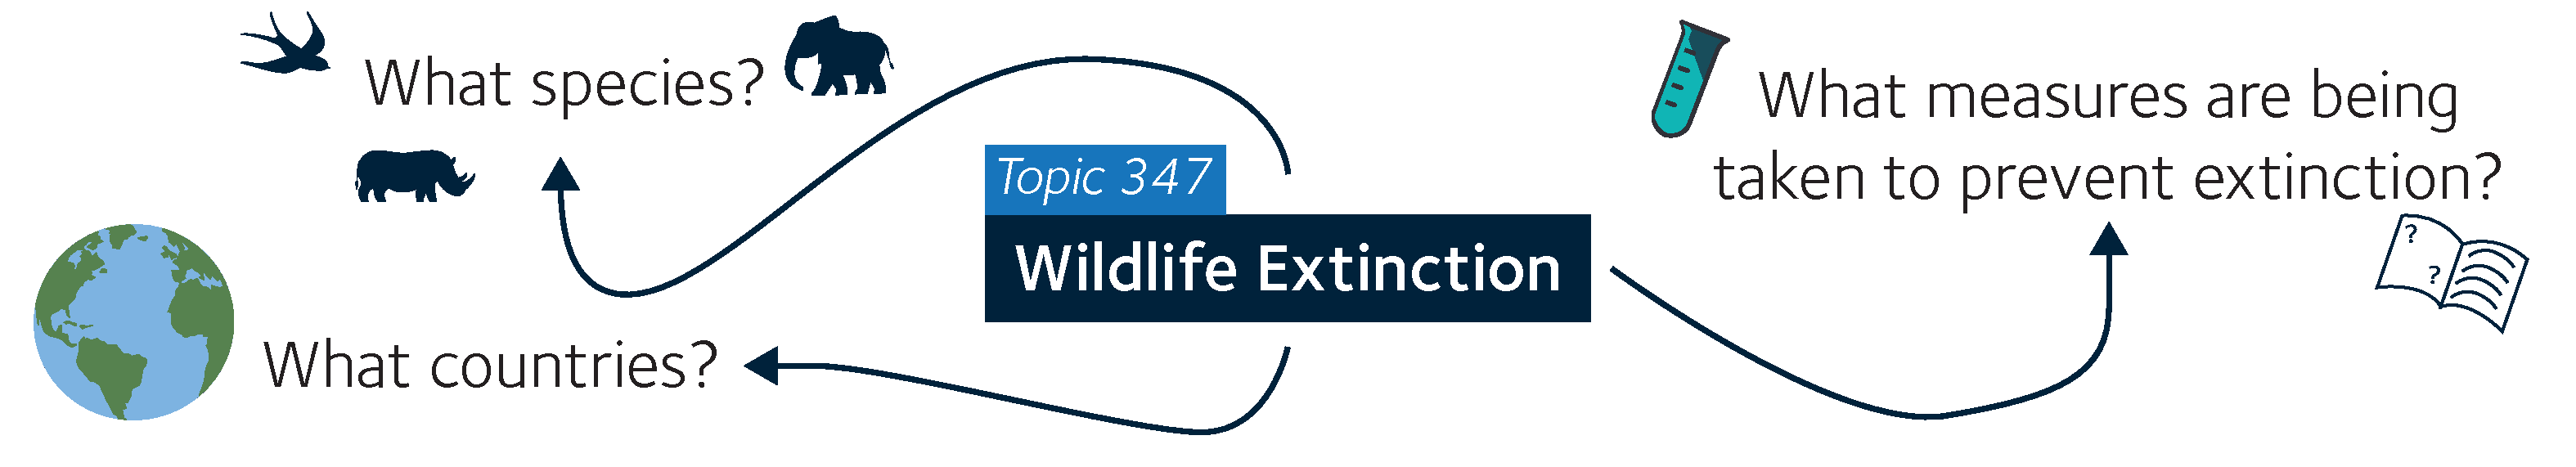
\includegraphics{figures/ch8-aspects_intro.pdf}}
    \label{fig:aspectsintro}
    \vspace{-5mm}
\end{figure}

While \emph{aspectual retrieval} has been heavily studied in the past (most prominently during the \emph{\gls{acr:trec} Interactive Tracks}~\citep{over2001trec}), there has been renewed interest in this type of search task. This is because it represents a novel context to explore the idea of \emph{``searching as learning''}~\citep{collins2017sal}. In this context, the goal of the system is to help the searcher learn about a topic~\citep{collins2017sal} -- and in doing so, the number of aspects the searcher finds provides an indication of how much they learned during the process~\citep{syed2017sal}. If the goal is to help searchers learn about a topic, then by returning results that are more diverse in nature and presenting a broader view of the topic, this \emph{should} assist searchers learn more about said topic. This reasoning suggests that employing \emph{diversification} will lead to an improved search and learning experience~\citep{syed2017sal}.

However, while there have been numerous diversification algorithms developed and proposed over the years\footnote{There are numerous examples of work on search result diversification, including measures such as \emph{Maximal Marginal Relevance (MMR)}~\citep{carbonell1998mmr}, and the \emph{xQuAD} framework~\citep{santos2010query_reformulations_diversification, santos2011intent}. Other studies in this area include works by~\cite{chen2006probabilistic_models} and~\cite{zhai2015subtopics}.}, the focus of the work reported in this chapter is on addressing the problem of intents, rather than how diversification affects complex search tasks, such as ad-hoc or aspectual retrieval. Thus, this chapter reports on:

\begin{itemize}
    \item{a user study, exploring how diversifying results (or not) affects the search behaviour and performance of searchers when undertaking different search tasks, from one of ad-hoc or aspectual retrieval (Section~\ref{sec:diversity:users}); and}
    \item{a simulated study, examining the various stopping strategies proposed in Chapter~\ref{chap:strategies}, utilising the~\gls{acr:csm}, perform under these tasks (Section~\ref{sec:diversity:simulated}).}
\end{itemize}

In particular, we use~\glsfirst{acr:ift}~\citep{pirolli1999ift} in this chapter -- outlined in Section~\ref{sec:stopping_background:models:theoretical:ift} on page~\pageref{sec:stopping_background:models:theoretical:ift} -- to derive a number of hypotheses, and thus ground our work. We begin this chapter however with a discussion of the prior work in the area, focusing upon aspectual retrieval, and a brief discussion of how~\gls{acr:ift} is used to provide us with a series of hypotheses about searcher behaviours across the different experimental conditions we trial.

\section{Background}
As discussed previously, a searcher will likely pose a varying number of queries (and~\glsplural{acr:serp}), and examine a number of documents (if any) before issuing a new query, or stopping their search altogether. The reasons for stopping are numerous. Stopping at a \emph{session level} can occur because:

\begin{itemize}
    \item{they have simply found enough information~\citep{prabha2007enough, dostert2009satisficing, hassan2013beyond_clicks};}
    \item{have run out of time~\citep{zach2005enough_is_enough}; or}
    \item{were dissatisfied with what they found~\citep{kiseleva2015serp_fails}; or}
    \item{simply gave up their search~\citep{diriye2012abandonment}.}
\end{itemize}

Numerous works have shown that different factors influence search behaviours -- this is demonstrated in Chapter~\ref{chap:snippets}, for instance, which showed how varying the length of result summaries influences behaviours. However, of particular relevance to this chapter is how different \emph{search tasks} influence a searcher's behaviours~\citep{kelly2015search_tasks}.

\subsection{Aspectual Retrieval}
An interesting search task that has not received much attention as of late is \emph{aspectual retrieval.} Aspectual retrieval is a type of search task that concerns the identification of different \emph{aspects} of a given topic. This task type differs from traditional ad-hoc retrieval in the sense that ad-hoc retrieval is concerned only with what constitutes a \emph{relevant} document to a given topic, rather than identifying relevant documents, and whether they are \emph{different} to what has been previously observed.

A relevant and different document will contain unseen aspects associated with the topic in question. With a graphical example provided at the beginning of this chapter, we now provide a further example to aid understanding. Consider the topic \emph{wildlife extinction} from the~\gls{acr:trec} 2005 Robust Track~\citep{voorhees2006trec_robust}. In an ad-hoc search task, if the searcher manages to find several documents concerning \texttt{Pandas in China}, these would all be considered relevant. However, for an aspectual retrieval task, where \emph{different} aspects must be found, the first document concerning \texttt{Pandas in China} is considered to be relevant/useful, and other aspects (in this case, the species of endangered animal) would need to be found, such as \texttt{Sumatran Rhinos in Malaysia}, \texttt{Crested Ibis in Japan}, etc.

Aspectual retrieval found significant traction in the \emph{\gls{acr:trec} Interactive Tracks}~\citep{over2001trec} from 1997-2002. The overarching goal of these tracks was to investigate searching, and an interactive task, by examining the processes involved, as well as the outcome~\citep{over2001trec}. Interaction was considered from the inaugural \emph{\gls{acr:trec}-1} in 1993~\citep{harman1993trec1}, where one group investigated interactive searching under the so-called \emph{interactive query mode} while undertaking an ad-hoc task. From \emph{\gls{acr:trec}-6} (1997) to \emph{\gls{acr:trec} 2002}, a substantial volume of research was directed towards the development of systems and search interfaces that:

\begin{itemize}
    \item{assisted searchers in exploring and retrieval various aspects of a topic, such as cluster-based and faceted interfaces that explicitly showed different aspects~\citep{mcdonald1998interactive, villa2009aspect_interface};}
    \item{provided tiles and stacks to organise documents~\citep{hearst1995tilebars, hearst1997texttiling, harper2006piling, iwata2012tilediversified}; and}
    \item{provided mechanisms to provide query suggestions that led to subjects following different search paths~\citep{kato2012query_suggestion, umemoto2016scentbar}.}
\end{itemize}

However, a disappointing conclusion from this initiative was that little difference was observed between such systems and the standard control systems (i.e. the traditional \emph{ten blue links}, as previously discussed in this thesis) -- both in terms of behaviour and performance~\citep{voorhees2005trec_book}.

As work shifted from aspectual retrieval to other areas, studies related to determining the intent of a searcher's query began to take hold, where the goal of this problem is to diversify the results retrieved with respect to the original query~\citep{rose2004understanding_user_goals}. Thus, this addresses the problem of \emph{ambiguity} for short, impoverished queries. This led to a series of diversification algorithms (and intent-aware evaluation measures), changing focus from the interface to the underlying algorithms and their evaluation measures. However, while there have been numerous studies investigating the effectiveness of diversification algorithms for the problem of query intents (e.g. one query, several possible interpretations), little work has looked at studying how such algorithms apply in the context of aspectual retrieval (e.g. one topic, many aspects). This is many due to the fact that most of these algorithms were developed \emph{after} the~\gls{acr:trec} Interactive Track finished in 2002.

Recently however, a growing interest in new, more complex and exploratory search tasks has taken hold. This is true in the aforementioned context of \emph{``searching as learning''}~\citep{collins2017sal}.~\cite{syed2017sal} hypothesised that diversifying the results presented to searchers would improve their learning efficiency, and that this would be observed by a change in vocabulary expressed in their queries. This work reported in this chapter motivates our interest examining the effects of diversification when considering the task of aspectual retrieval, where a searcher needs to learn about different aspects of a topic. To ground our work, we now consider how search behaviours are likely to be changed by generating a series of hypotheses from~\gls{acr:ift}.

\subsection{Tasks and Information Foraging Theory}
To motivate our hypotheses for this chapter, we can draw upon~\gls{acr:ift}~\citep{pirolli1999ift}, and the \emph{patch model} in particular, to ground our research and provide insights into how search behaviours may change. The patch model, as detailed in Section~\ref{sec:stopping_background:models:theoretical:ift}, provides a mechanism for predicting how long foragers will stay in a patch before moving onwards to the next. Using the established approach discussed previously -- where moving between patches is akin to issuing a new query, while staying within a patch considered examining a~\gls{acr:serp} and linked documents -- we can then make a series of predictions as to how searchers will behave under different experimental conditions.

\begin{figure}[t!]
    \centering
    \resizebox{1\hsize}{!}{
    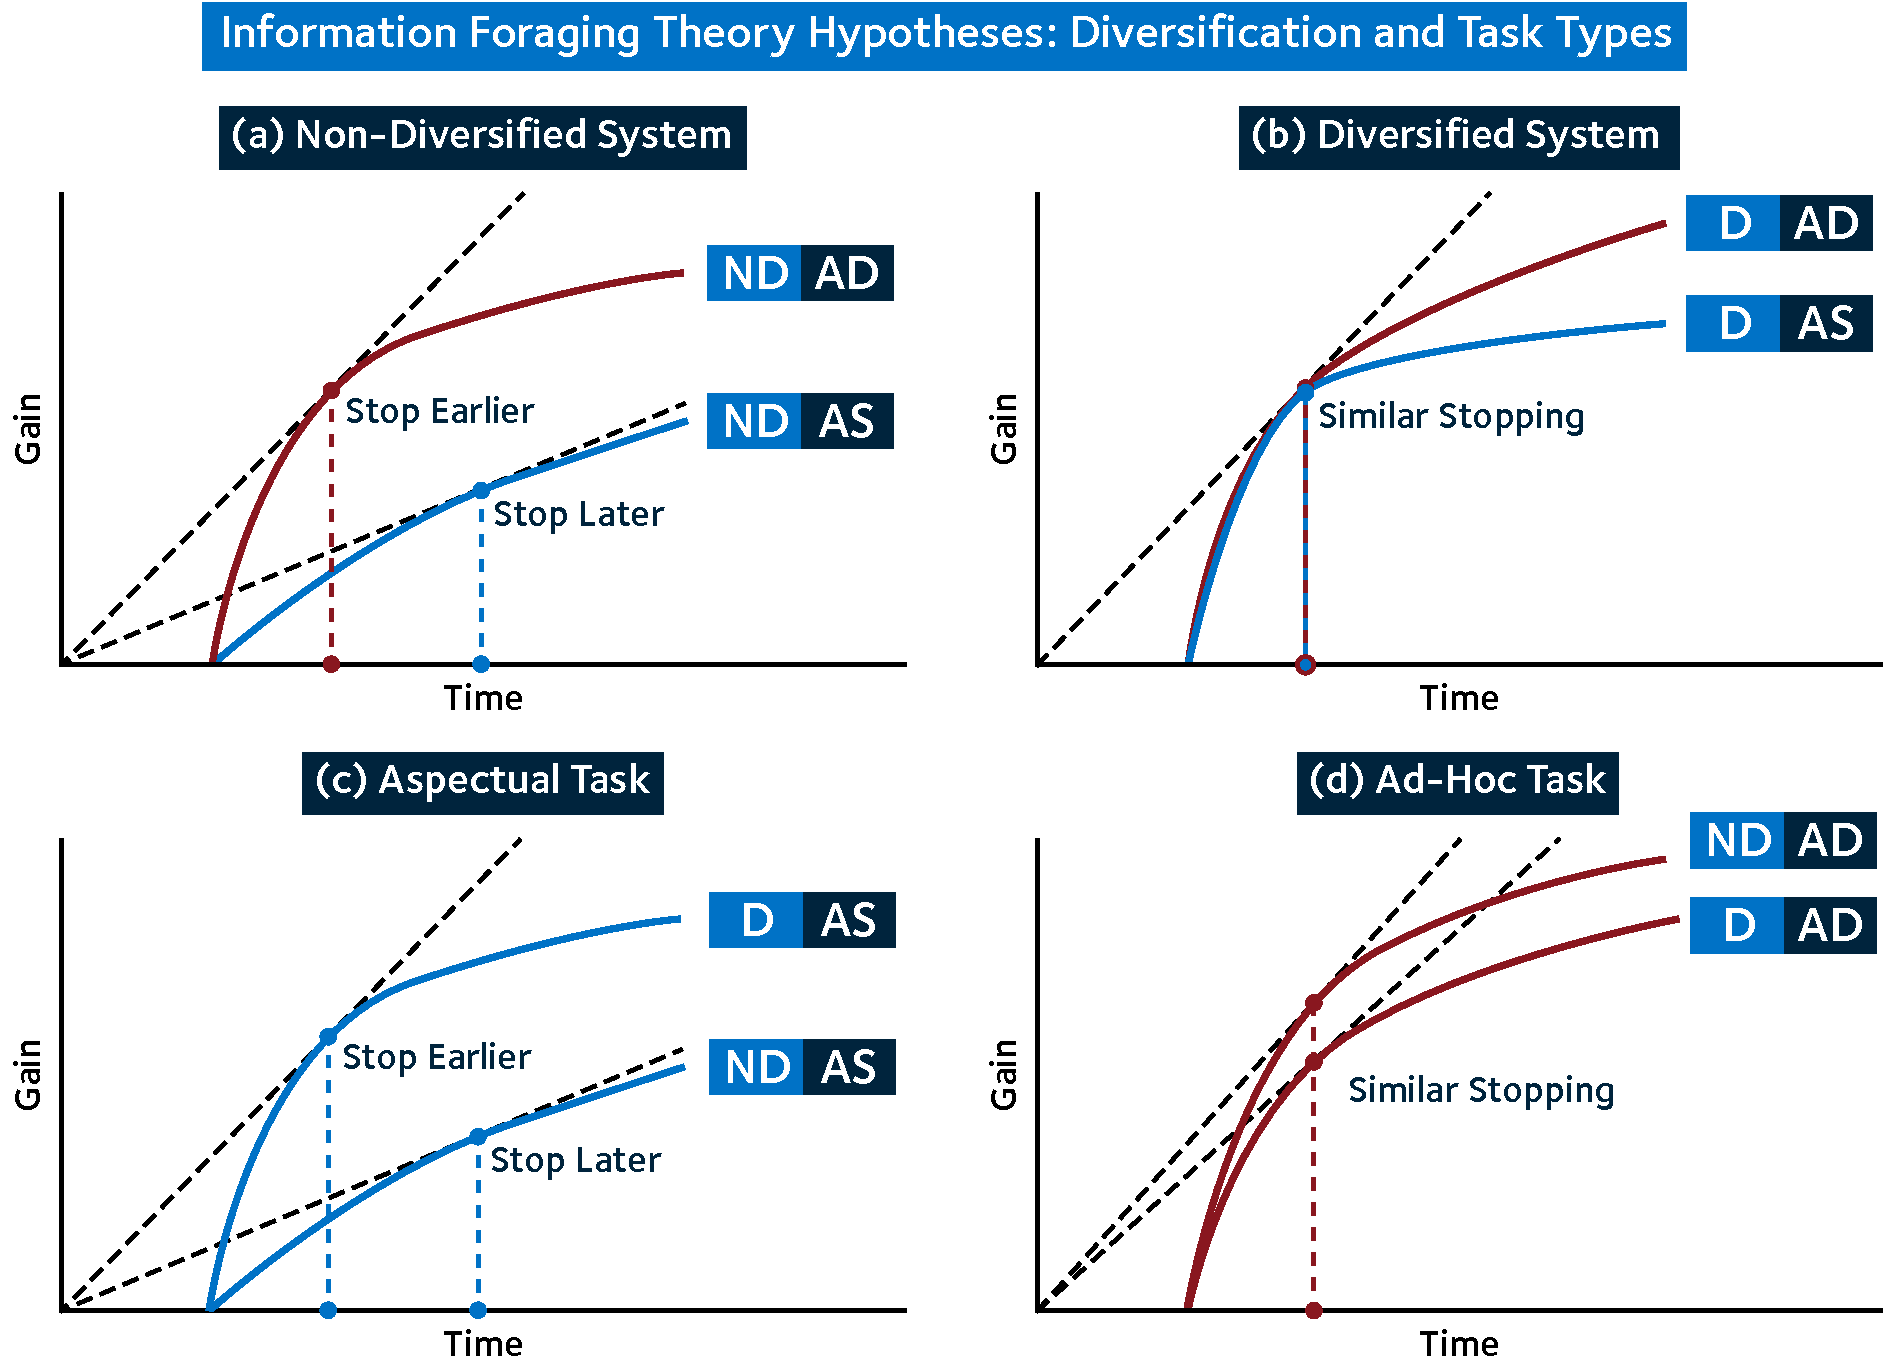
\includegraphics{figures/ch8-ift_theory_plots.pdf}}
    \caption[\gls{acr:ift} and Diversification: Hypothesis Illustrations]{Graphical illustrations of the hypotheses motivated by~\gls{acr:ift}, with each plot showing how stopping behaviour is likely to be affected when using a system that \emph{(a)} diversifies results and \emph{(b)} doesn't, and over \emph{(c)} aspectual and \emph{(d)} ad-hoc tasks. Refer to Section~\ref{sec:diversity:users:method:system} for details on the four different experimental conditions shown here, such as \dualbluebox{ND}{Ad}, for instance.}
    \label{fig:ift_theory}
\end{figure}

Discuss IFT, and then lead onto the hypotheses.

\section{Diversifying Search Results}\label{sec:diversity:users}
Including research questions, motivated by IFT


Following on from the aspectual retrieval part, the aim of this study is to better understand how searchers performance and search behaviour change when they undertake different types of search task, using search systems that diversify the ranked results, and those that do not. To ground this study, we first consider how search behaviour is likely to change by generating hypotheses from~\gls{acr:ift}.

\subsection{Research Questions and Hypotheses}

\subsection{Methodology}

\subsubsection{Search System and Conditions}\label{sec:diversity:users:method:system}

\subsubsection{Diversifying Search Results}

\subsubsection{Search Task}

\subsubsection{Additional Performance Measures}
$\alpha DCG$ and aspectual recall

\subsubsection{Crowdsourced Subjects}

\subsubsection{Post-Task Surveys}

\subsubsection{Post-Experiment Survey}

\subsection{Results}

\subsubsection{Interactions}

\subsubsection{Time-Based}

\subsubsection{Performance}

\subsubsection{User Experience}

\subsubsection{Gain over Time}

\subsection{Discussion}

\section{Simulated Analysis}\label{sec:diversity:simulated}

\section{Chapter Summary}